\documentclass[12pt,a4paper,oneside]{article}\usepackage[]{graphicx}\usepackage[]{color}
%% maxwidth is the original width if it is less than linewidth
%% otherwise use linewidth (to make sure the graphics do not exceed the margin)
\makeatletter
\def\maxwidth{ %
  \ifdim\Gin@nat@width>\linewidth
    \linewidth
  \else
    \Gin@nat@width
  \fi
}
\makeatother

\definecolor{fgcolor}{rgb}{0.345, 0.345, 0.345}
\newcommand{\hlnum}[1]{\textcolor[rgb]{0.686,0.059,0.569}{#1}}%
\newcommand{\hlstr}[1]{\textcolor[rgb]{0.192,0.494,0.8}{#1}}%
\newcommand{\hlcom}[1]{\textcolor[rgb]{0.678,0.584,0.686}{\textit{#1}}}%
\newcommand{\hlopt}[1]{\textcolor[rgb]{0,0,0}{#1}}%
\newcommand{\hlstd}[1]{\textcolor[rgb]{0.345,0.345,0.345}{#1}}%
\newcommand{\hlkwa}[1]{\textcolor[rgb]{0.161,0.373,0.58}{\textbf{#1}}}%
\newcommand{\hlkwb}[1]{\textcolor[rgb]{0.69,0.353,0.396}{#1}}%
\newcommand{\hlkwc}[1]{\textcolor[rgb]{0.333,0.667,0.333}{#1}}%
\newcommand{\hlkwd}[1]{\textcolor[rgb]{0.737,0.353,0.396}{\textbf{#1}}}%

\usepackage{framed}
\makeatletter
\newenvironment{kframe}{%
 \def\at@end@of@kframe{}%
 \ifinner\ifhmode%
  \def\at@end@of@kframe{\end{minipage}}%
  \begin{minipage}{\columnwidth}%
 \fi\fi%
 \def\FrameCommand##1{\hskip\@totalleftmargin \hskip-\fboxsep
 \colorbox{shadecolor}{##1}\hskip-\fboxsep
     % There is no \\@totalrightmargin, so:
     \hskip-\linewidth \hskip-\@totalleftmargin \hskip\columnwidth}%
 \MakeFramed {\advance\hsize-\width
   \@totalleftmargin\z@ \linewidth\hsize
   \@setminipage}}%
 {\par\unskip\endMakeFramed%
 \at@end@of@kframe}
\makeatother

\definecolor{shadecolor}{rgb}{.97, .97, .97}
\definecolor{messagecolor}{rgb}{0, 0, 0}
\definecolor{warningcolor}{rgb}{1, 0, 1}
\definecolor{errorcolor}{rgb}{1, 0, 0}
\newenvironment{knitrout}{}{} % an empty environment to be redefined in TeX

\usepackage{alltt}
\usepackage{amsmath,amsthm,amsfonts,amssymb}
\usepackage{pst-eucl,pstricks,pstricks-add}
\usepackage[utf8]{inputenc}
%\usepackage[latin1]{inputenc}
\usepackage[spanish,activeacute]{babel}
\usepackage[a4paper,margin=2.5cm]{geometry}
\usepackage{times}
\usepackage[T1]{fontenc}
\usepackage{titlesec}
\usepackage{color}
\usepackage{url}
\usepackage{float}
\usepackage{cite}
\usepackage{graphicx}
\usepackage{multicol}
\usepackage{lmodern}
\usepackage{setspace}
%\doublespace %para doble espacio
\onehalfspace %para espacio y medio
\newcommand{\code}[1]{\fcolorbox{blue!80}{gray!10}{#1}}
\parindent=0mm
\IfFileExists{upquote.sty}{\usepackage{upquote}}{}
\begin{document}
\begin{minipage}[d]{115mm}

\includegraphics[height=2.5cm, width=7.5cm]{logo_ult.pdf}
\end{minipage}
\begin{minipage}[d]{70mm}
\textsf{\textbf{\sc \tiny {\bf QUITO}: Fernando Oviedo E8-65 y José Barba}}\\
%\textsf{\textbf{\sc \tiny \qquad  Sector El Dorado}}\\
\textsf{\textbf{\sc \tiny {\bf CONTACTOS}: (02) 2 559-703 / (02) 2 602-560\\ Movistar: 0998428362 / 0998890021}}
\end{minipage}\\
\vspace{0.4cm}
%\rule[1mm]{150mm}{0.5mm}

\section{Quiénes somos ?}

Source Stat Lab (SSL) es una empresa Ecuatoriana con sede en Quito especializada en fomentar el avance del conocimiento, misma que presta sus servicios de entrenamiento y capacitación en el lenguaje de programación R para profesionales en todas sus verticales (investigación, docencia, empresarial). SSL brinda capacitación, reportería y consultoría estadística/matemática con el uso de herramientas de software libre como: R, RStudio, R Analytic Flow $\&$ LaTeX a empresas globales y locales, así como instituciones públicas.

\section{Historia}

SSL nació en Septiembre 2014 con el propósito de dar servicio y asesoramiento en investigaciones aplicadas que requieran de estudios estadísticos/matemáticos asociados a las mismas.

\section{Objetivos}

Entre los objetivos de SSL se encuentran:
\begin{itemize}
  \item Potenciar las actividades relacionadas con la Estadística que se llevan a cabo en varias universidades Ecuatorianas, así como ofrecer asesoramiento estadístico tanto a grupos de investigación como a particulares y empresas.  Dicho asesoramiento se complementa con cursos de formación adaptados a las necesidades y requerimientos del usuario.
  \item Fomentar el uso del software estadístico R en actividades académicas, profesionales e investigación.  
\end{itemize}
 
\section{Cursos}

Durante los últimos años, las nuevas tecnologías han permitido generar, almacenar y difundir grandes cantidades de información. Para poder extraer conocimiento y generar valor, hacen falta herramientas analíticas.\newline

Dado que la estadística es la herramienta determinante para la toma de decisiones y la obtención de conocimiento, SSL ofrece los siguientes cursos:
\begin{itemize}
  \item R Nivel Básico
  \item R Nivel Intermedio
  \item R Nivel Avanzado
  \item Gráficos con ggplot2
  \item Interfaces Web con Shiny
  \item Reportería Dinámica
%  \item Series Temporales
%  \item Minería de datos
%  \item Modelos lineales y de riesgo
\end{itemize}

%%% R Nivel Básico

\newpage

\begin{center}
{\bf \Large R Nivel Básico}
\end{center}

{\bf \large Descripción:}\newline
  
  El curso de R Nivel Básico tiene como objetivo principal proporcionar al estudiante una visión general del entorno del lenguaje de programación R y sus aplicaciones. Al final del curso, el estudiante se encontrará en la capacidad de crear sus propias funciones, importar y exportar datos. \newline
  
  El enfoque del curso se lo hará sobre el ámbito estadístico, sin embargo, lo anterior no resta méritos para que el estudiante amplie sus posibilidades en diversas áreas. Por tratarse de un curso inicial el estudiante recibirá abundante información la cual le permita profundizar de forma autónoma en la utilización del programa.\newline
  
{\bf \large Duración:}\newline
  20 Hrs.
  
{\bf \large Requisitos:}\newline
  Ninguno
  
{\bf \large Contenidos del curso:}

\begin{enumerate}
  \item {\Large Introducción}
  \begin{enumerate}
    \item[1.1] Funcionamiento
    \item[1.2] Ventajas
    \item[1.3] Desventajas
  \end{enumerate}
  \item {\Large Instalación y actualización}
  \begin{enumerate}
    \item[2.1] Programa R
    \item[2.2] Entorno de trabajo
    \item[2.3] Instalación de paquetes
    \item[2.4] Actualización de paquetes
    \item[2.5] Actualización de R
    \item[2.6] Obteniendo ayuda
  \end{enumerate}
  \item {\Large IDE}
  \begin{enumerate}
    \item[3.1] RStudio
    \item[3.2] R Analytic Flow
    \item[3.3] R Commander
  \end{enumerate}
  \item {\Large Estructura de datos}
    \begin{enumerate}
    \item[4.1] Vectores
    \item[4.2] Matrices
    \item[4.3] Arrays
    \item[4.4] Data Frames
    \item[4.5] Listas
    \item[4.6] Factores $\&$ Tablas
  \end{enumerate}
  \item {\Large Lectura y escritura de datos}
  \begin{enumerate}
    \item[5.1] Ingreso mediante el teclado
    \item[5.2] Lectura de archivos
    \item[5.3] Escritura de archivos
    \item[5.4] Accediendo a datos de la web
  \end{enumerate}
  \item {\Large Funciones}
    \begin{enumerate}
    \item[6.1] Funciones de R
    \item[6.2] Estructuras de control
    \item[6.3] Creación de funciones
    \item[6.4] Edición de funciones
    \item[6.5] Almacenamiento de funciones
  \end{enumerate}
\end{enumerate}

%%%& R Nivel Intermedio

\newpage

\begin{center}
{\bf \Large R nivel Intermedio}
\end{center}

{\bf \large Descripción:}\newline

El curso R nivel Intermedio tiene dos propósitos principales:
\begin{enumerate}
   \item Proporcionar al estudiante las principales herramientas de R utilizadas en la manipulación,
   tratamiento y depuración de la información de un conjunto de datos.
   \item Mostrar al estudiante una forma de optimizar las líneas de código tanto en tiempo de ejecución
   como en apariencia (códigos más compactos).
\end{enumerate}

Está dirigido a usuarios con un conocimiento básico de R. El curso se inicia analizando a detalle una amplia gama de R-funciones utilizadas en la práctica, mismas que permiten acelarar el tiempo de ejecución del código y a su vez  reducir el tiempo en la generación de grandes códigos que R ya los tiene implementados de forma más eficiente.\newline

Dentro de los temas a tratarse se encuentran las funciones \texttt{apply}, mismas que aplican una función a distintos objetos (vector, matriz, data frames, etc) evitando de esta forma la utilización de los típicos lazos iterativos {\bf for, while, etc} que por lo general resultan ser poco eficientes.\newline
  
{\bf \large Duración:}\newline
  20 Hrs.
  
{\bf \large Requisitos:}\newline
  R nivel Básico.
  
{\bf \large Contenidos del curso:}
\begin{enumerate}
   \item{Manipulación y depuración de bases de datos}
   \begin{enumerate}
      \item[1.1]{Unión de objetos y estructuras}
      \item[1.2]{Unión de bases de datos por columnas comunes}
      \item[1.3]{Valores perdidos y recodificación}
      \item[1.4]{Filtrado y ordenamiento de bases de datos}
      \item[1.5]{Discretización de variables}
      \item[1.6]{Muestras aleatorias}
      %\item[1.1]{Funciones paste(), cbind(), rbind()}
      %\item[1.2]{Funciones merge(), match(), grep(), etc.}
      %\item[1.3]{Funciones sort(), order()}
      %\item[1.5]{Funciones cut(), shingle()}
   \end{enumerate}
   \item{Aplicación de una función a cada elemento de un objeto}
   \begin{enumerate}
      \item[2.1]{Aplicación de una función a una matriz o arreglo}
      %Función apply()
      \item[2.2]{Aplicación de una función a una lista, data frame, vector}
      % Función lapply(), sapply()
      \item[2.3]{mapply() la versión multivariante de sapply()}
      \item[2.4]{Aplicación de una función a subgrupos de un vector}
      %Función tapply()
      \item[2.5]{Aplicación de una función a subgrupos de un data frame}
      %Función by()
      % rowSums(), colSums(), rowMeans(), and colMeans()
   \end{enumerate}
   \item{Funciones vectoriales}
   \begin{enumerate}
      \item[3.1]{Funciones vectoriales más utilizadas}
      %ifelse(), pmin(), pmax(), cumsum(), diff().
      \item[3.2]{Creación de funciones vectoriales}
      %Vectorize()
   \end{enumerate}
   \item{R-Funciones brillantes}
   \begin{enumerate}
      \item[4.1]{Funciones lógicas}
      %any(), all(), ifelse(), is.na(), noNA(x)
      \item[4.2]{Funciones matemáticas}
      %abs(), acos(), asin(), atan(), beta(), ceil(),
      %ceiling(), choose(), cos(), cosh(), digamma(), exp(), expm1(),
      %factorial(), floor(), gamma(), lbeta(), lchoose(), lfactorial(),
      %lgamma(), log(), log10(), log1p(), pentagamma(), psigamma(), round(),
      %signif(), sin(), sinh(), sqrt(), tan(), tanh(), tetragamma(),
      %trigamma(), trunc().
      \item[4.3]{Resumen de escalares}
      %mean(), min(), max(), sum(), sd(), and (for vectors) var().
      \item[4.4]{Resumen vectorial}
      %cumsum(), diff(), pmin(), and pmax().
      \item[4.5]{Buscando valores especificos en un objeto}
      %match(), self_match(), which_max(), which_min().
      \item[4.6]{Eliminación de registros duplicados}
      %duplicated(), unique().
   \end{enumerate}
\end{enumerate}


%%% R Nivel Avanzado

\newpage

\begin{center}
{\bf \Large R Nivel Avanzado}
\end{center}

{\bf \large Descripción:}\newline

El curso de R Nivel Avanzado tiene una visión general de varios temas de investigación avanzada, tales como: ambientes, programación orientada a objetos, big data, etc. El curso se encuentra dirigido a los estudiantes que ya tengan experiencia y conocimiento del programa estadístico R y que se encuentren dispuestos a obtener una perspectiva de mayor profundidad respecto a la programación R con visión en convertirse en un desarrollador.\newline

 % El enfoque del curso se lo hará sobre el ámbito estadístico, sin embargo, lo anterior no resta méritos para que el estudiante amplie sus posibilidades en diversas áreas. Por tratarse de un curso inicial el estudiante recibirá abundante información la cual le permita profundizar de forma autónoma en la utilización del programa.\newline
  
{\bf \large Duración:}\newline
  20 Hrs.
  
{\bf \large Requisitos:}\newline
  R Nivel Intermedio
  
{\bf \large Contenidos del curso:}

\begin{enumerate}
  \item {\Large Introducción}
  \begin{enumerate}
    \item[1.1] Cómo trabaja R
  \end{enumerate}
  \item {\Large Ambientes}
  \begin{enumerate}
    \item[2.1] Ambientes básicos
    \item[2.2] Recursividad
    \item[2.3] Funciones
    \item[2.4] Ambientes explícitos
  \end{enumerate}
  \item {\Large Programación orientada a objetos}
  \begin{enumerate}
    \item[3.1] Clases S3
    \item[3.2] Clases S4
    \item[3.3] Clases de referencia o R5
  \end{enumerate}
  \item {\Large Programación funcional}
    \begin{enumerate}
    \item[4.1] Funciones anónimas
    \item[4.2] Clausuras
    \item[4.3] Lista de funciones
  \end{enumerate}
  \item {\Large Evaluación no estándar}
  \begin{enumerate}
    \item[5.1] Captura de expresiones
    \item[5.2] Llamado desde otra función
    \item[5.3] Sustitución
  \end{enumerate}
  \item {\Large Expresiones}
    \begin{enumerate}
    \item[6.1] Estructura
    \item[6.2] Names
    \item[6.3] Calls
    \item[6.4] Parsing $\&$ Deparsing
  \end{enumerate}
    \item {\Large Big Data}
    \begin{enumerate}
    \item[7.1] Optimización de memoria
    \item[7.2] Carga de datos en disco
    \item[7.3] Manipulación de big data
  \end{enumerate}
\end{enumerate}


%%% Gráficos con ggplot2

\newpage

\begin{center}
{\bf \Large Gráficos estadísticos con ggplot2}
\end{center}

{\bf \large Descripción:}\newline

El objetivo del curso gráficos con {\bf ggplot2} es dotar al estudiante de importantes herramientas útiles en la generación de gráficos estadísticos de alta calidad y complejidad a través del paquete ggplot2, mismo que en la actualidad es uno de los paquetes gráficos de R más utilizados, la principal ventaja que presenta a diferencia de otros dispositivos gráficos es la utilización de un lenguaje estándar que permite describir la forma de visualización de manera sencilla (grámatica de gráficos), conocer dicha {\bf gramática de los gráficos} permite al usuario optimizar sus gráficos estándar y la vez generar gráficos totalmente nuevos e innovadores.

\begin{figure}[H]
\begin{center}
    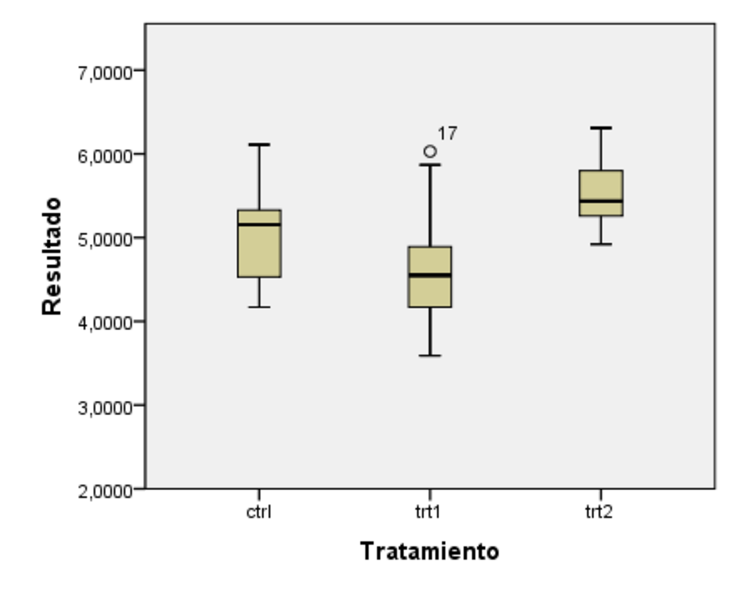
\includegraphics[width=0.41\textwidth]{DiagCajasSPSS.eps}
    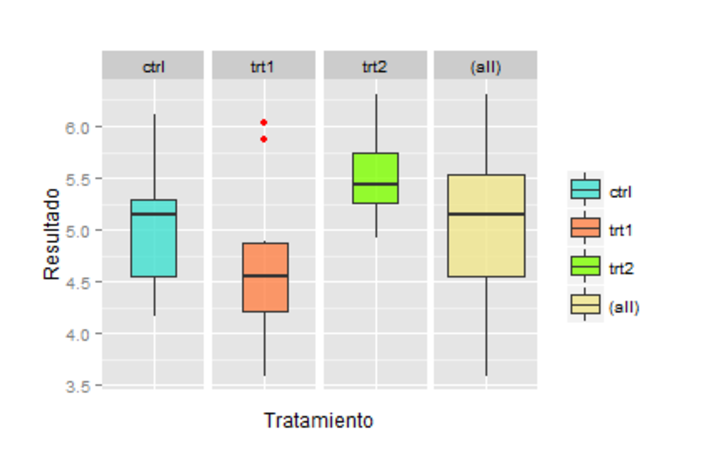
\includegraphics[width=0.55\textwidth]{DiagCajas.eps}
  \caption{Diagrama de cajas SPSS vs ggplot2.}
  \label{spssyg2}
\end{center}
\end{figure}

Entre los gráficos estadísticos generados con {\bf ggplot2} podemos enumerar los siguientes: histogramas, diagramas de densidad, de cajas y bigotes, de barras, de pastel, de dispersión, etc, adicionalmente, podemos crear {\bf mapas geográficos} en los cuales es posible presentar resúmenes estadísticos por región, provincia, etc (Estadística espacial). En la Figura 1 se muestra un claro ejemplo de la diferencia entre la calidad de un gráfico {\bf ggplot2} y de un gráfico realizado a través del programa estadístico clásico SPSS.\newline

{\bf \large Duración:}\newline
  20 Hrs.
  
{\bf \large Requisitos:}\newline
  R nivel básico.
  
{\bf \large Contenidos del curso:}
\begin{enumerate}
   \item Introducción e instalación del paquete
   \item La gramática de ggplot2
   \begin{enumerate}
   \item[2.1] Generación del primer gráfico ggplot2
   \end{enumerate}
   \item{Gráficos de distribución}
   \begin{enumerate}
      \item[3.1] Histogramas
      \item[3.2] Curvas de densidad
      \item[3.3] Diagrama de caja-bigotes
      \item[3.4] Multiples gráficos de distribución
   \end{enumerate}
   \item{Gráficos de líneas}
   \begin{enumerate}
      \item[4.1] Gráfico de líneas básicas
      \item[4.2] Gráfico de líneas múltiples
      \item[4.3] Apariencias de líneas (color, estilo, forma, etc).
   \end{enumerate}
   \item{Gráficos de dispersión}
   \begin{enumerate}
      \item[5.1] Gráfico de dispersión básico
      \item[5.2] Agrupación puntos con color, forma, etc.
      \item[5.3] Adición de líneas de ajuste de modelos de regresión
   \end{enumerate}
   \item{Mapas geográficos}
   \begin{enumerate}
      \item[6.1] Gráfico de mapa geografico básico
      \item[6.2] Adición de color, tipo de linea, etc. para cada provincia
      \item[6.3] Adición de resúmenes estadísticos por región, provincia, etc.
      \item[6.3] Adición de escalas de color
   \end{enumerate}
   \item{Formato del gráfico}
   \begin{enumerate}
      \item[7.1] Modificación de escala, color, letra, etc. de ejes
      \item[7.2] Modificación de posisión, color, letra, etc. de legendas
      \item[7.3] Modificación de margenes, color de fondo
   \end{enumerate}
   \item{Color en gráficos}
   \begin{enumerate}
      \item[8.1] Escala discreta de colores
      \item[8.2] Escala continua de colores
   \end{enumerate}
   \item{Facetas}
   \begin{enumerate}
      \item[9.1] Generación de gráficos por subgrupo de la data (variable discreta)
      \item[9.2] Generación de gráficos por dos subgrupos de la data (dos variables discretas)
   \end{enumerate}
\end{enumerate}


%%% Interface web con Shiny

\newpage

\begin{center}
{\bf \Large Interfaces de Usuario con Shiny}
\end{center}

{\bf \large Descripción:}\newline

Implementar un algoritmo en R permite disminuir considerablemente el tiempo de ejecución de una determinada tarea a diferencia de realizarla manualmente. El usuario de R siempre debe tener en mente que sus algoritmos serán utilizados por otros usuarios, entre ellos se debe considerar un pequeño porcentaje de usuarios que no poseen conocimiento suficiente del lenguaje R, es por esta razón que es necesario desarrollar interfaces gráficas mediante las cuales el usuario pueda ejecutar el algoritmo a través de botones y controladores (widgets), sin la necesidad de visualizar las líneas de código.\newline

\begin{figure}[H]
\begin{center}
     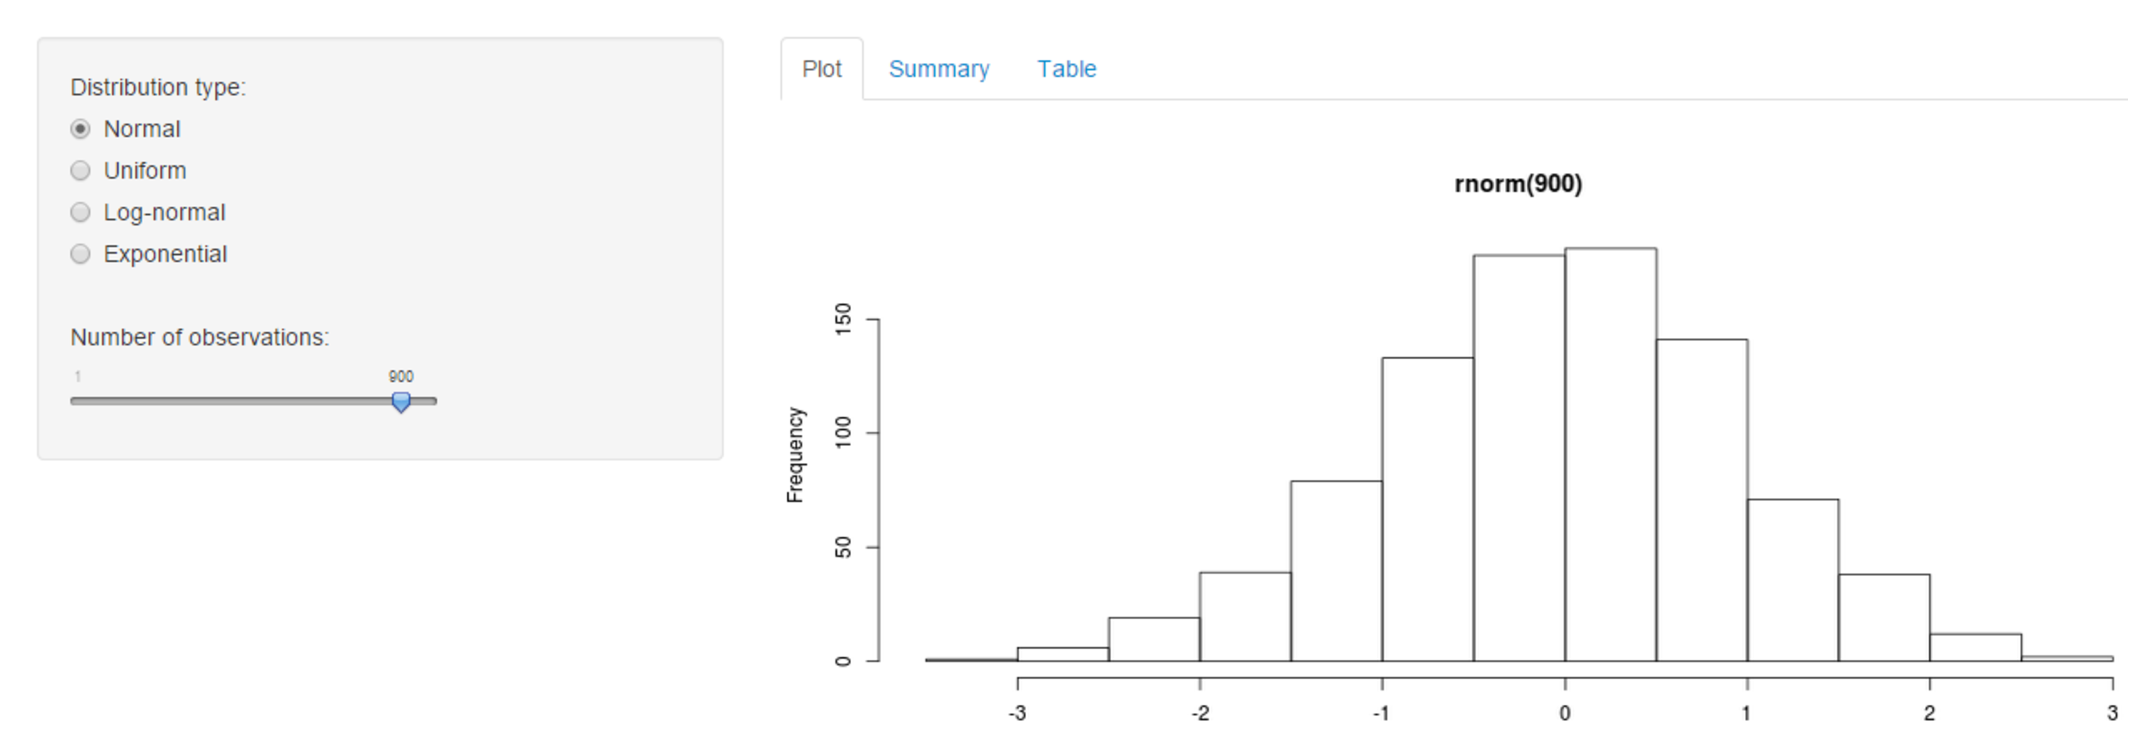
\includegraphics[width=0.8\textwidth]{gui_sim_var.eps}
  \caption{Simulación de variables aleatorias.}
  \label{simvar}
\end{center}
\end{figure}

El curso \emph{Interfaces de Usuario con Shiny} tiene como finalidad proveer al estudiante un conjunto de herramientas utilizadas en la generación de interfaces gráficas a través del paquete Shiny. Una vez que el estudiante logre comprender su estructura y funcionamiento resultará sencillo e intuitivo su uso. En la Figura 1 mostramos un ejemplo de una interfaz que simula un número de observaciones determinado de algunas distribuciones de probabilidad clásicas.\newline

{\bf \large Duración:}\newline
  20 Hrs.
  
{\bf \large Requisitos:}\newline
  R nivel básico.
  
{\bf \large Contenidos del curso:}

\begin{enumerate}
   \item{Introducción a Shiny}
   \begin{enumerate}
      \item[1.1]{Estructura de una aplicación}
      \item[1.2]{Ejecución de una aplicación}
      \item[1.3]{Ejemplos}
   \end{enumerate}
   \item{Diseño de la interfaz de usuario}
   \begin{enumerate}
      \item[2.1]{Construcción de la interfaz de usuario}
      \item[2.2]{Funciones y contenidos HTML}
      \item[2.3]{Formato de texto}
      \item[2.4]{Adición de imágenes y videos}
   \end{enumerate}
   \item{Añadir widgets de control (botones)}
   \begin{enumerate}
      \item[3.1]{Widgets de control básicos}
      \item[3.2]{Adición de widgets de control}
   \end{enumerate}
   \item{Objetos de salida reactiva}
   \begin{enumerate}
      \item[4.1]{Adición de un R objeto a la interfaz de usuario}
      \item[4.2]{Construcción de un objeto reactivo}
      \begin{itemize}
         \item Textos reactivos
         \item Gráficos reactivos
         \item Tablas reactivas, etc.
      \end{itemize}
   \end{enumerate}
   \item{Carga y descargo de archivos}
   \begin{enumerate}
      \item[5.1]{Carga de archivos y direcciones de archivos}
      \item[5.2]{Descarga de archivos de resultados}
   \end{enumerate}
   \item{Publicación de aplicaciones Shiny}
   \begin{enumerate}
      \item[6.1]{Ejecución de Interfaz mediante RStudio}
      \item[6.2]{Ejecución de Interfaz mediante un Navegador Web}
   \end{enumerate}
\end{enumerate}


%%% Reportería dinámica

\newpage

\begin{center}
{\bf \Large Repotería Dinámica}
\end{center}

{\bf \large Descripción:}\newline
  
  El curso de Reportería Dinámica tiene como finalidad integrar R con LaTeX, dichas herramientas permitirán generar reportes que se actualicen automáticamente a medida que los datos cambien. Esto facilita la elaboración de reportes evitando recurrir al famoso copy-paste de todos los resultados y gráficos de un programa a otro.\newline
  
  Al final del curso, el estudiante se encontrará en la capacidad de crear sus propios informes dinámicos en varios formatos digitales, mismos que eliminan la posibilidad de cometer errores de transcripción. \newline
  
{\bf \large Duración:}\newline
  20 Hrs.
  
{\bf \large Requisitos:}\newline
  R Nivel Básico
  
{\bf \large Contenidos del curso:}

\begin{enumerate}
  \item {\Large Introducción}
  \begin{enumerate}
    \item[1.1] Antecedente
    \item[1.2] Sweave
  \end{enumerate}
  \item {\Large Reportería}
  \begin{enumerate}
    \item[2.1] Buenas $\&$ malas prácticas
    \item[2.2] Restricciones
  \end{enumerate}
  \item {\Large Editores}
  \begin{enumerate}
    \item[3.1] RStudio
    \item[3.2] LyX
    \item[3.3] Otros editores
  \end{enumerate}
  \item {\Large Mi primer reporte}
    \begin{enumerate}
    \item[4.1] Configuraciones básicas
    \item[4.2] Knitr
    \item[4.3] LaTeX
    \item[4.4] Markdown
  \end{enumerate}
  \item {\Large Dinamizando la reportería}
  \begin{enumerate}
    \item[5.1] Syntaxis
    \item[5.2] Chunks
    \item[5.3] R Scripts
    \item[5.4] Tablas
    \item[5.5] Gráficos
    \item[5.6] Publicación en la web
  \end{enumerate}
  \item {\Large Cache}
    \begin{enumerate}
    \item[6.1] Implementación
    \item[6.2] Actualización
  \end{enumerate}
\end{enumerate}


\end{document}
